\documentclass{article}
\usepackage{amsmath}
\usepackage{graphicx}
\usepackage{listings}

\begin{document}

\section*{PROBLEM STATEMENT}
To implement the Mid-Point Ellipse Drawing Algorithm in C using OpenGL, and to draw an ellipse with a given center and semi-major and semi-minor axes on a 2D plane. The program will also draw the coordinate axes to visualize the ellipse in the context of a Cartesian coordinate system.

\section*{THEORY}
The Mid-Point Ellipse Drawing Algorithm is an efficient method to draw ellipses by determining the points of the ellipse using a decision parameter. It takes advantage of the ellipse's symmetry to reduce the number of points needed to be calculated. 

The algorithm is divided into two regions:
1. Region 1: Where the slope of the curve is less than 1.
2. Region 2: Where the slope of the curve is greater than or equal to 1.

The decision parameter helps in determining whether to move horizontally or diagonally to the next point based on the comparison of the current point's slope.

\section*{ALGORITHM}
\begin{enumerate}
    \item \textbf{Initialize}:
    \begin{itemize}
        \item Start with the initial point $(x, y) = (0, \text{ry})$.
        \item Calculate the initial decision parameter for Region 1: $d1 = \text{ry}^2 - (\text{rx}^2 \cdot \text{ry}) + (0.25 \cdot \text{rx}^2)$.
    \end{itemize}
    \item \textbf{Region 1}:
    \begin{itemize}
        \item While $2 \cdot \text{ry}^2 \cdot x < 2 \cdot \text{rx}^2 \cdot y$:
        \begin{itemize}
            \item Plot the point and its symmetrical points.
            \item Increment x by 1.
            \item If $d1 < 0$:
            \begin{itemize}
                \item $d1 = d1 + 2 \cdot \text{ry}^2 \cdot x + \text{ry}^2$
            \end{itemize}
            \item Else:
            \begin{itemize}
                \item Decrement y by 1.
                \item $d1 = d1 + 2 \cdot \text{ry}^2 \cdot x - 2 \cdot \text{rx}^2 \cdot y + \text{ry}^2$
            \end{itemize}
        \end{itemize}
    \end{itemize}
    \item \textbf{Region 2}:
    \begin{itemize}
        \item Calculate the initial decision parameter for Region 2: $d2 = (\text{ry}^2 \cdot (x + 0.5)^2) + (\text{rx}^2 \cdot (y - 1)^2) - (\text{rx}^2 \cdot \text{ry}^2)$.
        \item While $y \geq 0$:
        \begin{itemize}
            \item Plot the point and its symmetrical points.
            \item Decrement y by 1.
            \item If $d2 > 0$:
            \begin{itemize}
                \item $d2 = d2 + \text{rx}^2 - 2 \cdot \text{rx}^2 \cdot y$
            \end{itemize}
            \item Else:
            \begin{itemize}
                \item Increment x by 1.
                \item $d2 = d2 + 2 \cdot \text{ry}^2 \cdot x - 2 \cdot \text{rx}^2 \cdot y + \text{rx}^2$
            \end{itemize}
        \end{itemize}
    \end{itemize}
    \item \textbf{Termination}:
    \begin{itemize}
        \item The loop terminates when $y$ becomes less than 0.
    \end{itemize}
\end{enumerate}

\section*{FLOWCHART}
\begin{center}
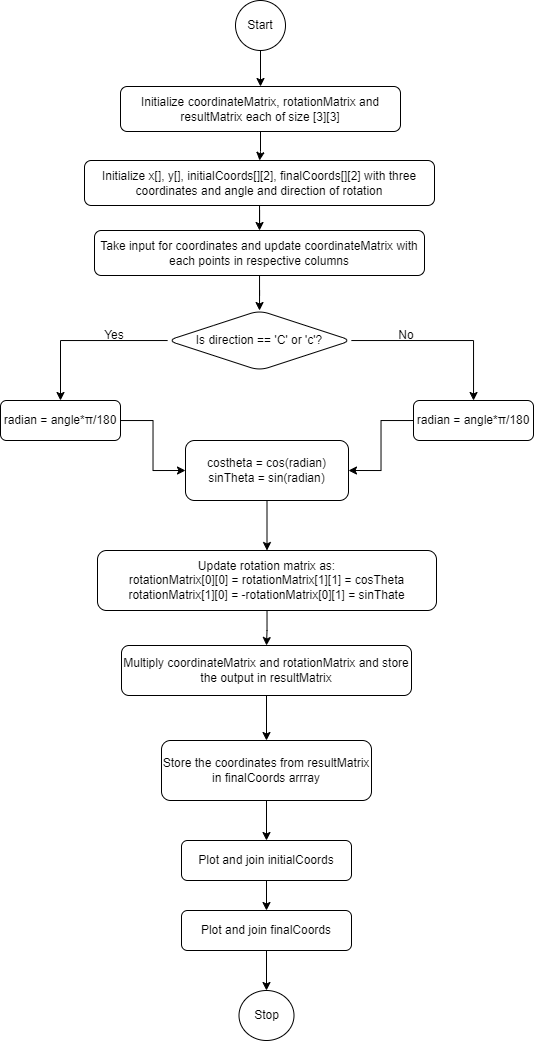
\includegraphics[width=0.7\textwidth]{flowchart.png}
\end{center}

\section*{SAMPLE I/O}
\textbf{Input:}
\begin{verbatim}
Enter the coordinates of the center of the ellipse (xc, yc): 0 0
Enter the semi-major axis length (rx): 100
Enter the semi-minor axis length (ry): 50
\end{verbatim}

\textbf{Output:}
An ellipse is drawn with center $(0, 0)$, semi-major axis length $100$, and semi-minor axis length $50$ on a window with coordinate axes displayed.

\section*{DISCUSSIONS}
\begin{itemize}
    \item \textbf{Accuracy}: The Mid-Point Ellipse Drawing Algorithm accurately plots the ellipse points based on the decision parameters, ensuring the correct shape of the ellipse.
    \item \textbf{Efficiency}: The algorithm is efficient due to its use of symmetry and decision parameters to reduce the number of calculations.
    \item \textbf{Applications}: This algorithm is used in various applications such as computer graphics, game development, and CAD software where ellipses need to be rendered.
\end{itemize}

\section*{CONCLUSION}
The Mid-Point Ellipse Drawing Algorithm is a powerful and efficient method for drawing ellipses on raster displays. By utilizing decision parameters and symmetry, it ensures accurate and visually correct ellipses. The implementation using OpenGL demonstrates the algorithm's capability to draw ellipses with any given center, semi-major, and semi-minor axes and visualize the coordinate axes.

\end{document}
